\documentclass[11pt,a4paper]{article}

\usepackage[T1]{fontenc}
\usepackage[utf8]{inputenc}
\usepackage[english]{babel}
\usepackage{lmodern}
%\usepackage{circuitikz}
\usepackage{color}
\usepackage{wrapfig}
\usepackage{placeins}
\usepackage{subfigure}
\usepackage{tabu}
\usepackage{fullpage}
\usepackage[squaren]{SIunits}
\usepackage{graphicx}
%\usepackage[pdftex]{graphicx}
\usepackage{epstopdf}
\usepackage{epsfig}
\usepackage{hyperref}
\usepackage{tikz}
\usepackage{tikz-qtree}
\usepackage{eurosym}
%\usepackage{chemist}
\usepackage{amsmath}
\usepackage{amssymb}
\usepackage{mathrsfs}
\usepackage{dsfont}% use $\mathds{1}$
\newcommand{\C}{\mathbb{C}}
\newcommand{\N}{\mathbb{N}}
\newcommand{\Z}{\mathbb{Z}}
\newcommand{\R}{\mathbb{R}}
\newcommand{\red}{\textcolor{red}}
\newcommand{\dis}{\displaystyle}
\newcommand{\dr}{\partial}
\newcommand{\txt}{\text}
\newcommand{\td}{\todo[inline]}
\newcommand{\ttt}{\texttt}
\newcommand{\itt}{\textit}

\usepackage{algorithm}
\usepackage{todonotes}
\usepackage[noend]{algpseudocode}

%\newtheorem{theoreme}			     {Théorème}	[chapter]
%\newtheorem{proposition}[theoreme]	 {Proposition}	
%\newtheorem{corollaire}	  [theoreme]	 {Corollaire}	
%\newtheorem{lemme}	      [theoreme]  {Lemme}		
%\newtheorem{definition}	         {Définition}[chapter]
%\theoremstyle{definition}
%\newtheorem{exemple}			     {Exemple}	[chapter]
%\newtheorem{contreexemple}[exemple]{Contre-exemple}
%\newtheorem{probleme}	             {Probl\`eme}[chapter]

\usepackage{listings}
\usepackage{textcomp}
\definecolor{listinggray}{gray}{0.9}
\definecolor{lbcolor}{rgb}{0.9,0.9,0.9}
\lstset{
	backgroundcolor=\color{lbcolor},
	tabsize=4,
	rulecolor=,
	language=matlab,
        basicstyle=\scriptsize,
        upquote=true,
        aboveskip={1.5\baselineskip},
        columns=fixed,
        showstringspaces=false,
        extendedchars=true,
        breaklines=true,
        prebreak = \raisebox{0ex}[0ex][0ex]{\ensuremath{\hookleftarrow}},
        frame=single,
        showtabs=false,
        showspaces=false,
        showstringspaces=false,
        identifierstyle=\ttfamily,
        keywordstyle=\color[rgb]{0,0,1},
        commentstyle=\color[rgb]{0.133,0.545,0.133},
        stringstyle=\color[rgb]{0.627,0.126,0.941},
}

\DeclareMathOperator{\e}{e}

\title{Titre}
\author{David Weicker}
\date{\today}

\begin{document}
\tabulinesep=1.2mm
\begin{center}
\hrule
\begin{tabular}{c}
\\[0.005cm]
\Large{SF2521: Homework Assignment 3}\\[0.3cm] %THIS IS THE TITLE
\textsc{Thomas} Garrett  \& \textsc{Weicker} David\\[0.2cm]
$\text{6}^{\text{th}}$ November 2015\\[0.2cm] %THIS IS THE DATE
\end{tabular}
\hrule
\end{center}

\section{Well–posedness and von Neumann analysis}
In this section, we consider the $2\pi$-periodic Cauchy problems
\begin{align*}
u_t &= \alpha u_{xx} + \beta u_{xxxx} \\
u(x,0) &= sin(x)
\end{align*}


\subsection{Well-posed for $\alpha>0$ and $\beta = 0$}
We now show that the problem is well-posed in the $L_2$ -norm for for $\alpha>0$ and $\beta = 0$.
\begin{align*}
u_t &= \alpha u_{xx}
u(x,0) &= sin(x)
\end{align*} 
It is seen immediately that we now have the one dimensional heat equation. The solution to this problem is well documented and, given our initial condition, we have $u(x,t) = sin(x)e^{-at}$  



\subsection{Ill-posed for $\beta>0$}


\subsection{Stability for $\alpha>0$ and $\beta=0$}
We wish to derive a condition on $\Delta t$ which guarantees stability in the max norm for a scheme using central difference in time and forward Euler in space. 

\section{Shallow water equations, dissipation and dispersion}
In this section, we will further analyze the shallow water equations, already discussed in homework 2. 

Here, we will use the Lax-Wendroff as well as the  McCormack's method defined by :
$$u_j^* = u_j^n - \frac{\Delta t}{\Delta x} (f(u_{j+1}^n)-f(u_j^n))$$
$$u_j^{n+1} = \frac{1}{2}(u_j^n+u_j^*) - \frac{\Delta t}{2\Delta x}(f(u_j^*)-f(u_{j-1}^*))$$

\subsection{Order of accuracy of the method}
We will now try to compute the order of accuracy of McCormack's scheme. To do this, we will plug the solution of the PDE into the scheme and use Taylor's expansion. Let $u(x,t)$ be the solution of the following PDE : 
$$u_t + (f(u))_x = 0$$

Using Taylor's expansion, the left-hand side of the scheme is :
$$u_j^{n+1} = u(x_j,t_n + \Delta t) = u(x_j,t_n) + \Delta t u_t(x_j,t_n) + \frac{\Delta t^2}{2} u_{tt}(x_j,t_n) + \frac{\Delta t^3}{6} u_{ttt}(x_j,t_n) + O(\Delta t^4)$$

Let us now compute $f(u_{j+1}^n-f(u_j^n)$. Using Taylor expansion, we have :
\begin{align*}
f(u(x_j+\Delta x,t_n))-f(u(x_j,t_n)) &= (f(u(x_j,t_n)) + \Delta x (f
\end{align*}

\subsection{Numerical solution with McCormack's scheme}
We will now present the numerical solution of the shallow water equations using McCormack's scheme and compare it with the one obtained with Lax-Wendroff. The code can be found at the end of the report.

Figures \ref{mc01} and \ref{mc02} present the solution for two different values of the ratio $\frac{\Delta t}{\Delta x}$. For both those plots, the number of point in the x-direction is $N=100$.

\begin{figure}
\begin{center}
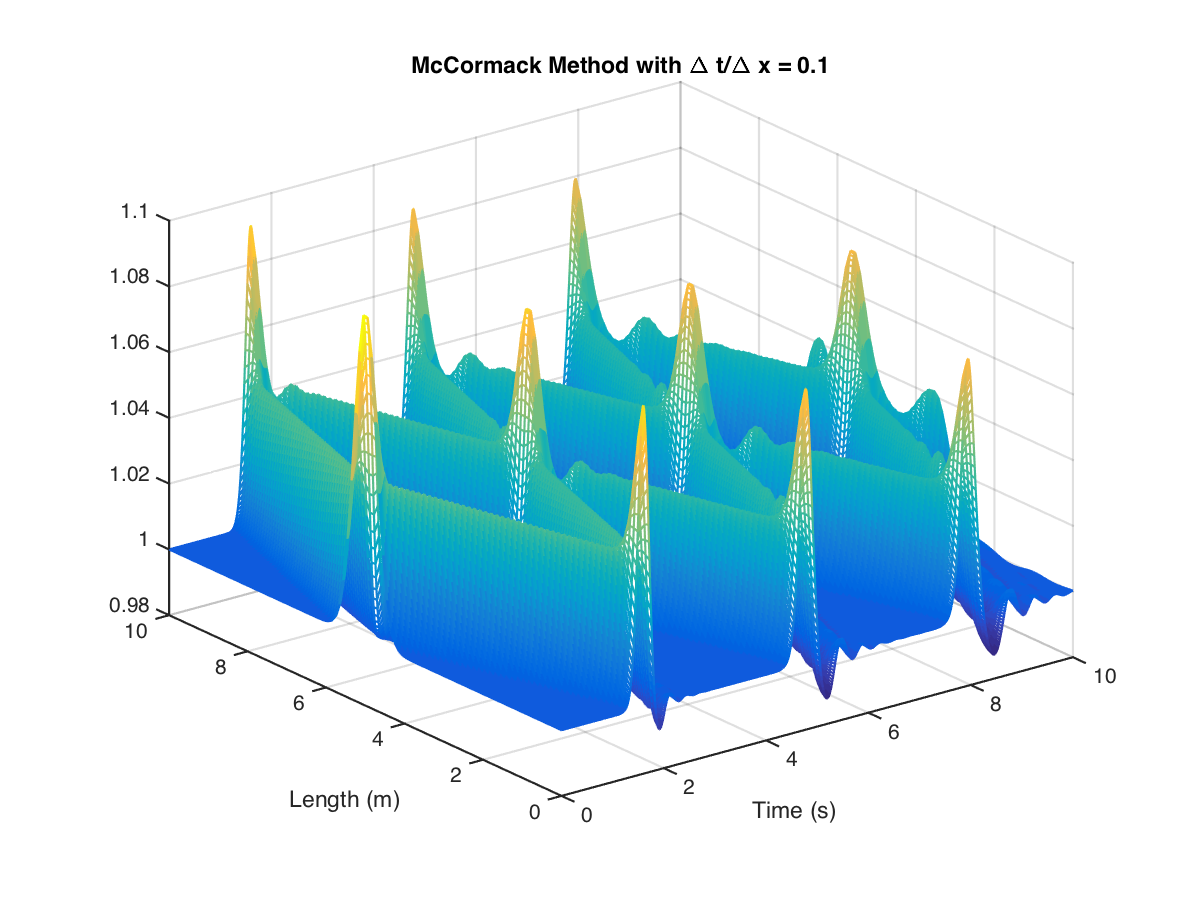
\includegraphics[scale=0.6]{mccormack01.eps}
\caption{Solution for $\frac{\Delta t}{\Delta x}= 0.1$ with McCormack's scheme}
\label{mc01}
\end{center}
\end{figure}

\begin{figure}
\begin{center}
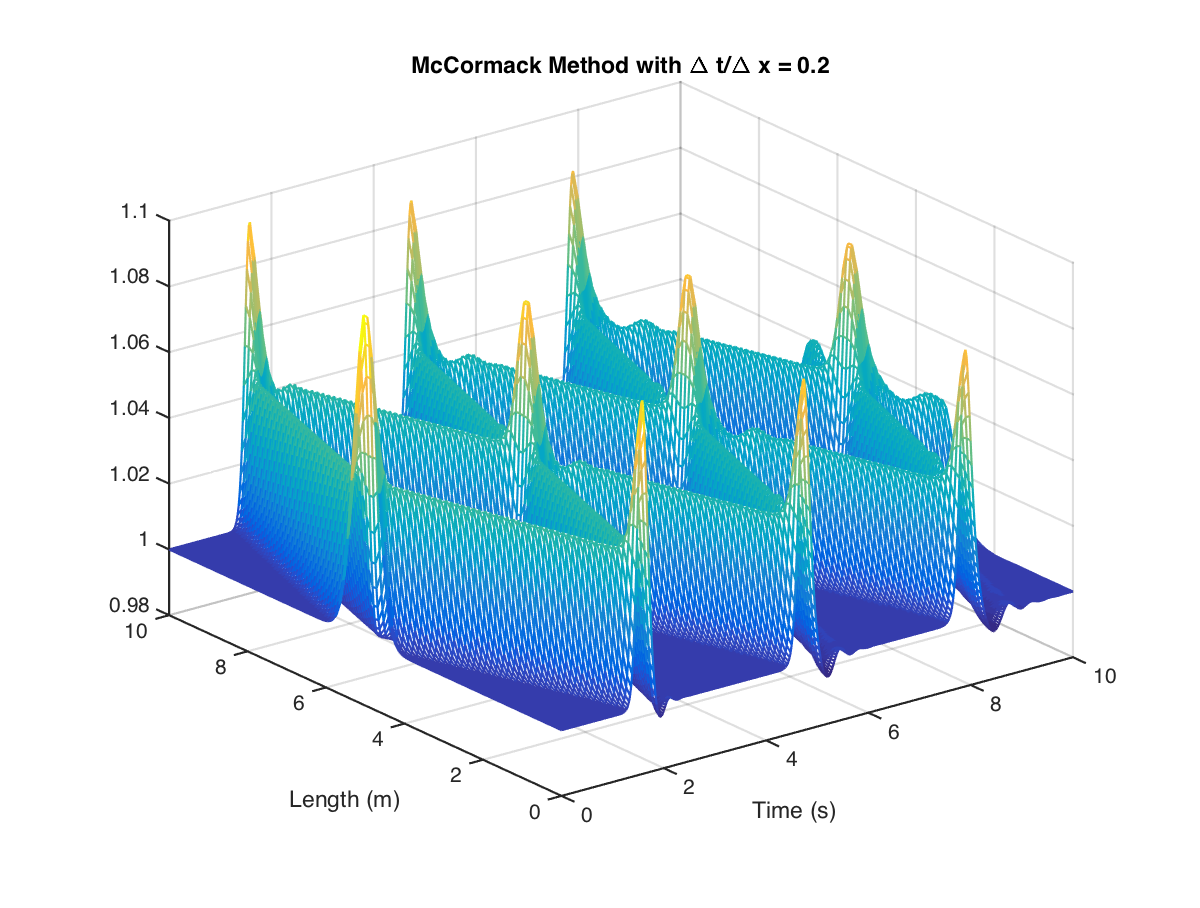
\includegraphics[scale=0.6]{mccormack02.eps}
\caption{Solution for $\frac{\Delta t}{\Delta x}= 0.2$ with McCormack's scheme}
\label{mc02}
\end{center}
\end{figure}

There are several remarks to make. We can first see dispersion errors at the boundary and more generally where the gradients are steep. We can also see that those dispersion errors tend to increase with time. This is particularly visible when the ratio is equal to 0.1.

To better understand the effects of discretization, we also have figure \ref{mc200}, where the ratio is also equal to 0.2 but with now $N=200$, i.e. the spatial grid has been refined. 
\begin{figure}
\begin{center}
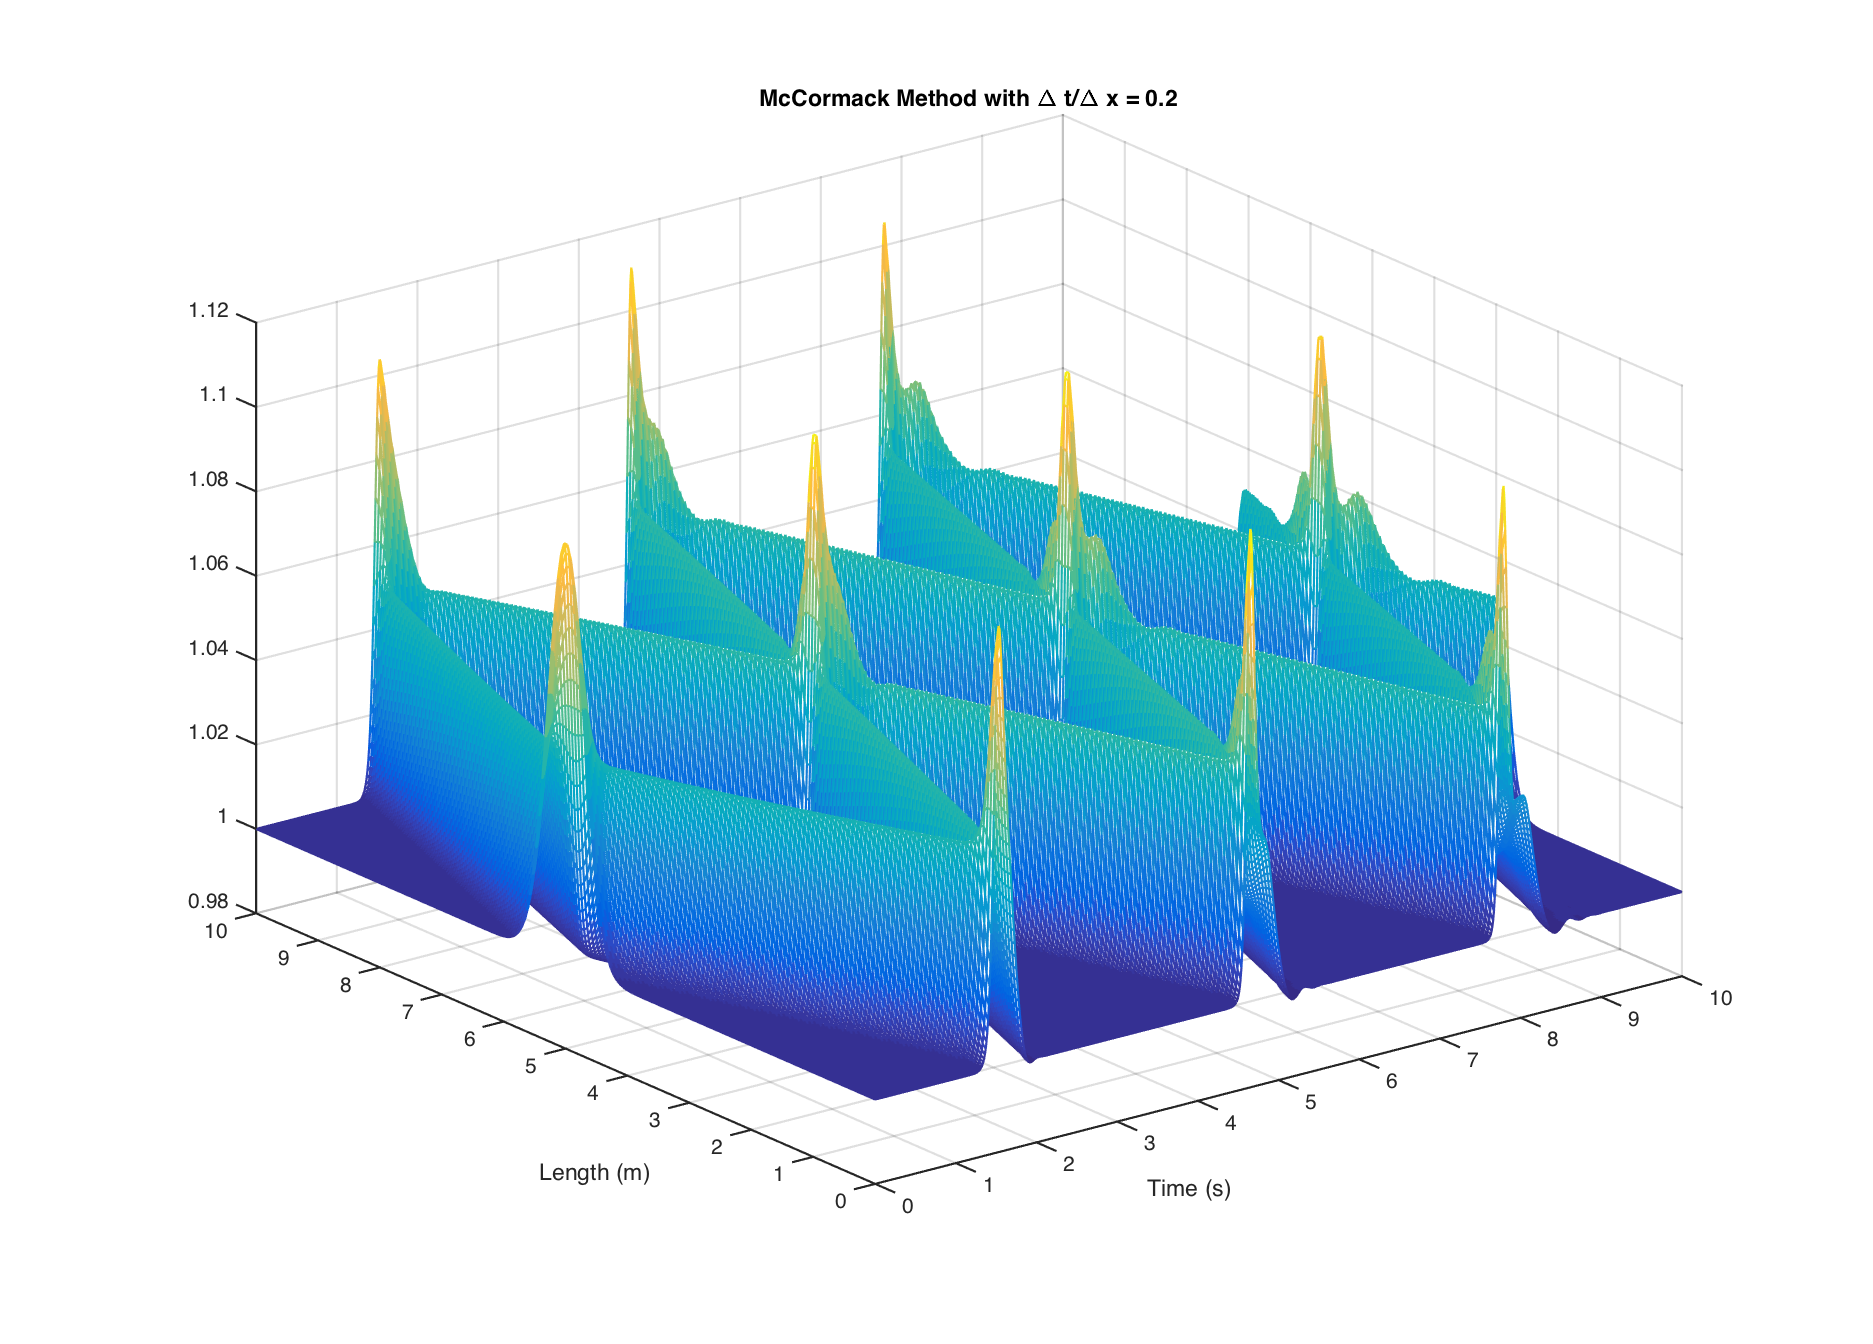
\includegraphics[scale=0.5]{mccormack02200.eps}
\caption{Solution for $\frac{\Delta t}{\Delta x}= 0.2, N=200$ with McCormack's scheme}
\label{mc200}
\end{center}
\end{figure}

Here, we can see that we have smaller dispersion errors at the boundary. However, this is not true around the peaks. There, the dispersion errors look the same or even a bit bigger.

Finally, it is interesting to compare the two methods. With Lax-Wendroff we did not have any dispersion errors as we have with McCormack. However, Lax-Wendroff dissipation errors and the smaller the ratio $\frac{\Delta t}{\Delta x}$ is, the bigger the dampening of the wave we can observe. This does not happen with McCormack, we have no dampening whatever the ratio. Our last remark will be that with both method, the numerical solution is unstable when the ration is larger than 0.3.



\end{document}